\def\hide{0}

%!Tex Root = ../main.tex
% ./Design.tex
% ./Deklarationen.tex
% ./Vorbereitung.tex
% ./Aufgabe1.tex
% ./Aufgabe2.tex
% ./Aufgabe3.tex
% ./Appendix.tex

% https://tex.stackexchange.com/questions/83101/option-clash-for-package-xcolor
% [table]
% https://tex.stackexchange.com/questions/14336/latex-beamer-presentation-package-169-aspect-ratio
% https://tex.stackexchange.com/questions/203045/latex-error-option-clash-for-package-hyperref
% https://stackoverflow.com/questions/3637129/how-can-i-top-align-the-content-of-a-fragile-frame-in-a-latex-beamer-presentat
% https://latex-beamer.com/faq/place-content-frame/
\documentclass[aspectratio=169, hyperref={colorlinks=true, allcolors=PrimaryColor}, c]{beamer}
% t to position content at the top: https://tex.stackexchange.com/questions/9889/positioning-content-at-the-top-of-a-beamer-slide-by-default

% ┌──────────┐
% │ Packages │
% └──────────┘

% \usepackage[margin=1.5cm, headheight=12.5pt]{geometry}
\usepackage[ngerman]{babel}

\usepackage{lipsum}

\usepackage{multirow}

\usepackage[parfill]{parskip}
% % https://latexref.xyz/bs-par.html
\setlength{\parskip}{0.4cm} % space between paragraphs
% \usepackage{setspace}

\usepackage[export]{adjustbox}

% as beamer itself already provides these functionalities, there is no need to load hyperref, color, graphicx, graphics
% \usepackage{graphicx}

% % https://tex.stackexchange.com/questions/48509/insert-list-of-figures-in-the-table-of-contents
% \usepackage[nottoc]{tocbibind}

% % colorbox stuff
\usepackage{tcolorbox}
\usepackage{tikz}
% \usepackage{pgfplots}
% \usepackage{pgfgantt}

\usepackage{tikzit}
\input{graph_theory.tikzstyles}

\usetikzlibrary {arrows.meta,positioning}
\usetikzlibrary{graphs}
\tcbuselibrary{skins}
\tcbuselibrary{breakable}
\usetikzlibrary{patterns}
\usetikzlibrary{shadings}
\usetikzlibrary{mindmap, backgrounds, calc}
\tcbuselibrary{theorems}
% \tcbuselibrary{listings}
% https://tex.stackexchange.com/questions/550052/command-parboxrestore-has-changed
\tcbuselibrary{minted}
\tcbset{listing engine=minted}
\tcbuselibrary{raster}

% % https://tex.stackexchange.com/questions/547950/highlight-labeled-lines-of-code-with-minted
% % \usepackage{refcount}

% \usepackage{cleveref}

\usepackage[style=numeric]{biblatex}
\addbibresource{./Library/My Library.bib}

% \usepackage{pdfpages}
% https://tex.stackexchange.com/questions/94845/problems-with-toprule-and-midrule-in-a-table


\usepackage{tabularray}
\usepackage{booktabs} % for table rules
% % \usepackage{tabulary}
% % https://tex.stackexchange.com/questions/395554/command-rowcolors-from-colortbl-does-not-work-as-expected

\usepackage{nicematrix}
% \usepackage{tabularx}
% \usepackage{array}
% \usepackage{multirow}
% \usepackage{amssymb}

% https://tex.stackexchange.com/questions/157389/how-to-center-column-values-in-a-table
% \newcolumntype{P}[1]{>{\centering\arraybackslash}p{#1}}

% https://stackoverflow.com/questions/2888817/footnotes-for-tables-in-latex
% \usepackage{tablefootnote}

% https://tex.stackexchange.com/questions/8625/force-figure-placement-in-text
% \usepackage{float}

% https://tex.stackexchange.com/questions/219445/line-break-in-texttt
\usepackage{seqsplit}
\newcommand{\seqtt}[1]{{\scriptsize\texttt{\seqsplit{#1}}}}
\newcommand{\smalltt}[1]{{\small\texttt{#1}}}
\newcommand{\tinytt}[1]{{\tiny\texttt{#1}}}
\newcommand{\scripttt}[1]{{\scriptsize\texttt{#1}}}

% https://tex.stackexchange.com/questions/358292/creating-a-subcounter-to-a-counter-i-created
\usepackage{chngcntr}

% https://tex.stackexchange.com/questions/18870/defining-an-new-itemize-like-environment-where-itemfoo-passes-foo-to-a-macro
\usepackage{ifmtarg}


% https://stackoverflow.com/questions/1061112/eliminate-space-before-beginitemize
% https://tex.stackexchange.com/questions/31505/trouble-combining-enumitem-and-beamer
% https://tex.stackexchange.com/questions/325003/given-enumitem-beamer-incompatibility-how-do-i-adjust-the-indent-of-the-enume
% https://tex.stackexchange.com/questions/455692/beamer-presentation-with-itemize-exceed-text-capacity

% https://tex.stackexchange.com/a/263470
\usepackage{microtype}

% https://tex.stackexchange.com/questions/165178/nameref-hyperref-evaluating-counter-instead-of-section-name
% \usepackage{nameref}

% https://stackoverflow.com/questions/1078370/subfigs-of-a-figure-on-multiple-pages
% \usepackage{subfig}

% https://tex.stackexchange.com/questions/186981/is-there-a-subsubsubsection-command
% https://tex.stackexchange.com/questions/130795/how-can-i-number-sections-below-subsection-in-latex
% \setcounter{secnumdepth}{5}

% % https://stackoverflow.com/questions/2854299/getting-subsection-to-list-in-table-of-contents-in-latex
\setcounter{tocdepth}{4}

% https://tex.stackexchange.com/questions/369421/how-to-have-a-figure-going-over-several-pages
% TODO: set hypcap = true when compiling for the last time
% https://tex.stackexchange.com/questions/132611/change-color-of-figure-caption-text
\usepackage[labelfont={color=SecondaryColor, it}, textfont={it}]{caption}
% hypcap=false
\usepackage{subcaption}

% https://tex.stackexchange.com/questions/7210/label-and-caption-without-float
\DeclareCaptionType{codecaption}[Code][Codeverzeichnis]
% https://tex.stackexchange.com/questions/449677/spaces-in-newenvironment
\newenvironment{code}{\bigskip\captionsetup{type=codecaption}}{\medskip}

% https://texblog.net/latex-archive/uncategorized/prevent-floating-image-figure-table/
% \newcommand\captionof[1]{\def\@captype{#1}\caption}
% \usepackage{capt-of}

% \usepackage{formal-grammar}

% newfloat package
% \SetupFloatingEnvironment{floatgrammar}{name=Grammatik}

% \renewcommand{\downplay}[0]{\rowstyle{\color{gray!90!black}}}
% \newcommand{\removed}[0]{\rowstyle{\color{red}}}

% https://tex.stackexchange.com/questions/26637/how-do-you-get-mathbb1-to-work-characteristic-function-of-a-set
% \usepackage{bbm}
% \usepackage{newtxmath}

% https://tex.stackexchange.com/questions/27843/level-of-boldness-changeable
\usepackage[bold=1]{xfakebold}

% \newcommand{\footnoteurl}[1]{\href{#1}{Link}\footnote{\url{#1}.}}

% https://www.namsu.de/Extra/befehle/Cases.html
\usepackage{mathtools}

\usepackage{breqn}

% https://tex.stackexchange.com/questions/479632/newcommand-combine-optional-star-and-optional-parameter
% \usepackage{xparse}
\tcbuselibrary{xparse}

% https://texfaq.org/FAQ-twooptarg
\usepackage{xargs}

% emojis
\usepackage{tikzsymbols}

\usepackage{algorithm2e}

% https://tex.stackexchange.com/questions/237974/hide-section-numbering-but-keep-labeling
% reference titles of sections
% \usepackage[usetoc]{titleref}

% % https://tex.stackexchange.com/questions/531/what-is-the-best-way-to-use-quotation-mark-glyphs
\usepackage{csquotes}

% https://tex.stackexchange.com/questions/326527/colored-blocks-for-numbered-theorems-in-beamer
\usepackage{etoolbox}% new package to be loaded

% https://jansoehlke.com/2010/06/strikethrough-in-latex/
% \usepackage[normalem]{ulem}
% \usepackage{cancel}

% get checkmark
\usepackage{amsmath}
\usepackage{breqn}

% change font size
\usepackage{anyfontsize}

\usepackage{etoolbox}

%!Tex Root = ../main.tex
% ./Packete.tex
% ./Deklarationen.tex
% ./Vorbereitung.tex
% ./Aufgabe1.tex
% ./Aufgabe2.tex
% ./Aufgabe3.tex
% ./Bonus.tex

\newtoggle{gabriella}
% \toggletrue{gabriella}
\togglefalse{gabriella}
\iftoggle{gabriella}{
  \def\gabriella{1}
}{
  \def\gabriella{0}
}

% ┌──────────────────────┐
% │ Beamer Configuration │
% └──────────────────────┘

\usetheme{default}
\useoutertheme{infolines}

% ┌─────────────────────┐
% │ Color Configuration │
% └─────────────────────┘

% % https://latexdraw.com/how-to-draw-venn-diagrams-in-latex/
% as beamer itself already provides these functionalities, there is no need to load hyperref, color, graphicx, graphics
% \usepackage{xcolor}

\iftoggle{gabriella}{
  \definecolor{PrimaryColor}{HTML}{F80016}
  \definecolor{PrimaryColorDimmed}{HTML}{FF949E}
  \definecolor{SecondaryColor}{HTML}{F36622}
  \definecolor{SecondaryColorDimmed}{HTML}{F9B797}
}{
  \definecolor{PrimaryColor}{HTML}{0B64A0}
  \definecolor{PrimaryColorDimmed}{HTML}{A2D7F3}
  \definecolor{SecondaryColor}{HTML}{6FC1EC}
  \definecolor{SecondaryColorDimmed}{HTML}{CEEAF9}
}
\colorlet{BoxColor}{gray!10!white}

\setbeamercolor{normal text}{%
  fg=black,
  bg=white
}
\setbeamercolor{alerted text}{%
  fg=SecondaryColor,
}

% \setbeamercolor{example text}{%
%   fg=PrimaryColor,
% }

\setbeamercolor{structure}{fg=SecondaryColor}

\setbeamercolor{frametitle}{fg=PrimaryColor}
\setbeamercolor{framesubtitle}{fg=SecondaryColor}

\setbeamercolor{title}{fg=PrimaryColor, bg=BoxColor}
\setbeamercolor{subtitle}{fg=SecondaryColor}

% https://github.com/josephwright/beamer/blob/main/base/themes/color/beamercolorthemedefault.sty
% https://github.com/josephwright/beamer/blob/main/base/themes/outer/beamerouterthemeinfolines.sty
\setbeamercolor{author in head/foot}{fg=PrimaryColor, bg=PrimaryColorDimmed}
\setbeamercolor{title in head/foot}{fg=SecondaryColor, bg=SecondaryColorDimmed}
\setbeamercolor{date in head/foot}{fg=PrimaryColor, bg=PrimaryColorDimmed}

\setbeamercolor{palette primary}{fg=PrimaryColor,bg=PrimaryColorDimmed}
\setbeamercolor{palette secondary}{fg=SecondaryColor,bg=SecondaryColorDimmed}
\setbeamercolor{palette tertiary}{fg=PrimaryColor,bg=PrimaryColorDimmed}
\setbeamercolor{palette quaternary}{fg=PrimaryColor,bg=PrimaryColorDimmed}

\setbeamercolor{block title}{fg=white, bg=PrimaryColor}
\setbeamercolor{block body}{fg=black, bg=BoxColor}

\setbeamercolor{block title example}{fg=white, bg=PrimaryColor}
\setbeamercolor{block body example}{fg=black, bg=BoxColor}

\setbeamercolor{block title alerted}{fg=white, bg=SecondaryColor}
\setbeamercolor{block body alerted}{fg=black, bg=BoxColor}

% https://tex.stackexchange.com/questions/326527/colored-blocks-for-numbered-theorems-in-beamer
% https://tex.stackexchange.com/questions/87216/how-to-change-the-color-of-the-text-in-a-theorem-in-beamer/87219#87219
\AtBeginEnvironment{theorem}{% set of commands to be added
    \setbeamercolor{block title}{fg=white,bg=PrimaryColor}% colors to change
    \setbeamercolor{block body}{fg=black,bg=PrimaryColorDimmed}% colors to change
}

\AtBeginEnvironment{proof}{%
    \setbeamercolor{block title}{fg=white,bg=SecondaryColor}
    \setbeamercolor{block body}{fg=black,bg=SecondaryColorDimmed}
}

% https://tex.stackexchange.com/questions/87133/changing-the-color-of-itemize-item-in-beamer
\setbeamercolor{itemize item}{fg=SecondaryColor}
\setbeamercolor{itemize subitem}{fg=SecondaryColor}
\setbeamercolor{itemize subsubitem}{fg=SecondaryColor}

\setbeamercolor{enumerate item}{fg=SecondaryColor}
\setbeamercolor{enumerate subitem}{fg=SecondaryColor}
\setbeamercolor{enumerate subsubitem}{fg=SecondaryColor}

% ┌─────────────────────────┐
% │ Titlepage Configuration │
% └─────────────────────────┘

\newcommand{\titlesecond}{Tutorat 2}
\newcommand{\subtitlesecond}{RETI, Huffman-Kodierung}
\newcommand{\group}{
  \if\gabriella0{
      Gruppe 9
  }\else{
      Gruppe 4
  }\fi
}
\newcommand{\type}{
  \group\\[-0.25cm]
  \rule{6cm}{0.1mm}
}
\newcommand{\authorsecond}{
\if\gabriella0{
  Jürgen Mattheis
}\else{
  Gabriella Frank
}\fi
}
\newcommand{\mail}{
\if\gabriella0{
  (\href{mailto://juergmatth@gmail.com}{juergmatth@gmail.com})
}\else{
  (\href{mailto://gabriella-frank@web.de}{gabriella-frank@web.de})
}\fi
}
\newcommand{\moreinformation}{
\begin{columns}[t]
  \begin{column}{0.5\textwidth}
    \raggedright
    \small
    \emph{Vorlesung von:}

    Prof. Dr. Scholl
  \end{column}
  \begin{column}{0.5\textwidth}
    \raggedleft
    \small
    \emph{Übungsgruppenbetreuung:}

    Tobias Seufert
  \end{column}
\end{columns}
}
\newcommand{\institutesecond}{Universität Freiburg}
\newcommand{\datesecond}{\today}
% \logo{\includegraphics[height=0.5cm]{./figures/logo.png}}

\newcommand{\lehrstuhl}{Lehrstuhl für Rechnerarchitektur}

\defbeamertemplate*{title page2}{default}[1][]{
  \vbox{}
  \vfill
  \begingroup
    \centering
    \begin{beamercolorbox}[sep=8pt,center,#1]{title}
      \usebeamerfont{title}\titlesecond\par%
      \ifx\subtitlesecond\@empty%
      \else%
        \vskip0.25em%
        {\usebeamerfont{subtitle}\usebeamercolor[fg]{subtitle}\subtitlesecond\par}%
      \fi%
    \end{beamercolorbox}%
    \begin{beamercolorbox}[sep=8pt,center,#1]{institute}
       \type
    \end{beamercolorbox}
    \begin{beamercolorbox}[sep=8pt,center,#1]{author}
      \if\gabriella0{
          \usebeamerfont{author}\emph{Präsentator:}\\ \authorsecond\\\mail
      }\else{
          \usebeamerfont{author}\emph{Präsentatorin:}\\ \authorsecond\\\mail
      }\fi
    \end{beamercolorbox}
    \vspace{-1em}
    \begin{beamercolorbox}[sep=8pt,center,#1]{institute}
      \moreinformation
    \end{beamercolorbox}%\vskip1em
    \begin{beamercolorbox}[sep=8pt,center,#1]{date}
      \usebeamerfont{date}\emph{\datesecond}
    \end{beamercolorbox}
    \begin{beamercolorbox}[sep=8pt,center,#1]{institute}
      \usebeamerfont{institute}\institutesecond, \lehrstuhl
    \end{beamercolorbox}
    {\usebeamercolor[fg]{titlegraphic}\inserttitlegraphic\par}
  \endgroup
  \vfill
}

\makeatletter
\def\titlepagesecond{\usebeamertemplate*{title page2}\@thanks}
\makeatother

\setbeamertemplate{title page2}[default][colsep=-4bp,rounded=true,shadow=true]

% ┌───────────────────────┐
% │ Footline and Headline │
% └───────────────────────┘

% https://github.com/josephwright/beamer/blob/main/base/themes/outer/beamerouterthemeinfolines.sty
\makeatletter
\setbeamertemplate{footline}{%
  \leavevmode%
  \hbox{%
    \begin{beamercolorbox}[wd=.333333\paperwidth,ht=2.25ex,dp=1ex,center]{author in head/foot}%
      \usebeamerfont{author in head/foot}\authorsecond % \expandafter\ifblank\expandafter{\beamer@shortinstitute}{}{~~(\insertshortinstitute)}
    \end{beamercolorbox}%
    \begin{beamercolorbox}[wd=.333333\paperwidth,ht=2.25ex,dp=1ex,center]{title in head/foot}%
      \usebeamerfont{title in head/foot}\titlesecond,\enspace\group
    \end{beamercolorbox}%
    \begin{beamercolorbox}[wd=.333333\paperwidth,ht=2.25ex,dp=1ex,leftskip=2ex,rightskip=2ex,sep=0pt]{date in head/foot}%
      \hfill%
      \usebeamerfont{author in head/foot}%
      \institutesecond
      \hfill%
      \usebeamercolor[fg]{page number in head/foot}%
      \usebeamerfont{page number in head/foot}%
      \usebeamertemplate{page number in head/foot}%
    \end{beamercolorbox}
  }%
  \vskip0pt%
}
\makeatother

\setbeamertemplate{headline}{%
\leavevmode%
  \hbox{%
    % https://tex.stackexchange.com/questions/85439/custom-headline-in-latex-beamer
    \begin{beamercolorbox}[wd=\paperwidth,ht=2.5ex,dp=1.125ex]{palette quaternary}%
      \textcolor{PrimaryColor}{\insertsectionnavigationhorizontal{\paperwidth}{\hskip0pt plus1filll}{\hskip0pt plus1filll}}
    \end{beamercolorbox}%
  }
}

% https://tex.stackexchange.com/questions/44983/beamer-removing-headline-and-its-space-on-a-single-frame-for-plan-but-keepin
\newenvironment{withoutheadline}{
  \setbeamertemplate{headline}{%
  \leavevmode%
    \hbox{%
      \begin{beamercolorbox}[wd=\paperwidth,ht=2.5ex,dp=1.125ex]{palette primary}%
      \end{beamercolorbox}%
    }
  }
}{}

\newenvironment{withoutfootline}{
  \setbeamertemplate{footline}{%
  \leavevmode%
    \hbox{%
      \begin{beamercolorbox}[wd=\paperwidth,ht=2.5ex,dp=1.125ex]{palette secondary}%
      \end{beamercolorbox}%
    }
  }
}{}

% ┌──────────────────────┐
% │ Layout Configuration │
% └──────────────────────┘

\setbeamertemplate{blocks}[rounded][shadow=true]

% https://tex.stackexchange.com/questions/578098/number-of-figure-in-beamer
\setbeamertemplate{caption}[numbered]

% \setbeamertemplate{sidebar canvas left}{}
\setbeamersize{sidebar width right=1.5cm}
\setbeamertemplate{sidebar right}{%
  \vspace*{\fill}
  \if\gabriella0{
    
\includegraphics[width=1.5cm, height=\paperheight]{./figures/background.png}
  }\else{
    
\includegraphics[width=1.5cm, height=\paperheight]{./figures/backgrounda.png}
  }\fi
  \vspace*{\fill}
}

\newcommand{\insertsectionHEAD}{%
	\expandafter\insertsectionHEADaux\insertsectionhead}
	\newcommand{\insertsectionHEADaux}[3]{\LARGE#3
}

\AtBeginSection[] {
  \begingroup
  \setbeamercolor{background canvas}{bg=PrimaryColorDimmed}

  \setbeamertemplate{sidebar right}{%
    \vspace*{\fill}
    \if\gabriella0{
        
\includegraphics[width=1.5cm, height=\paperheight]{./figures/background.png}
    }\else{
        
\includegraphics[width=1.5cm, height=\paperheight]{./figures/backgrounda.png}
  }\fi
    \vspace*{\fill}
  }

  \begin{frame}
    \centering
    \textcolor{PrimaryColor}{\insertsectionHEAD}
  \end{frame}
  \endgroup
}

% TOC at beginning of each section
% \AtBeginSection[]{
%   \begin{frame}{Gliederung}
%     \tableofcontents[currentsection]
%   \end{frame}
% }

% https://tex.stackexchange.com/questions/87133/changing-the-color-of-itemize-item-in-beamer
\setbeamertemplate{itemize item}[triangle]
\setbeamertemplate{itemize subitem}[triangle]
\setbeamertemplate{itemize subsubitem}[triangle]
% square, circle, triangle, \rightTextArrow

% ┌────────────────────┐
% │ Font Configuration │
% └────────────────────┘

\setbeamerfont{title}{size=\LARGE}
\setbeamerfont{date}{size=\footnotesize}
\setbeamerfont{author}{size=\small}
\setbeamerfont{institute}{size=\small}
\setbeamerfont{subtitle}{size=\large}

\setbeamerfont{frametitle}{size=\LARGE}
\setbeamerfont{framesubtitle}{size=\large}

\setbeamerfont{normal text}{size=\tiny}
\setbeamerfont{itemize/enumerate body}{size=\scriptsize}
\setbeamerfont{itemize/enumerate subbody}{size=\scriptsize}
\setbeamerfont{itemize/enumerate subsubbody}{size=\scriptsize}

% ┌───────────┐
% │ Resources │
% └───────────┘

% - latex beamer templates als Inspiration: https://github.com/benjamin-weiss/hsrmbeamertheme/blob/master/beamerthemehsrm.sty
% - inspiration: https://github.com/martinbjeldbak/ultimate-beamer-theme-list
% - https://github.com/matze/mtheme
% - https://github.com/josephwright/beamer/blob/main/base/themes/color/beamercolorthemedefault.sty
  % - different templates switch
% - https://github.com/josephwright/beamer/blob/main/base/themes/color/beamercolorthemecrane.sty
% - https://github.com/josephwright/beamer/blob/main/base/themes/color/beamercolorthemebeetle.sty
% - https://www.cpt.univ-mrs.fr/~masson/latex/Beamer-appearance-cheat-sheet.pdf
% - (https://git.imp.fu-berlin.de/raup90/swp_2019/-/blob/master/presentation/fu-beamer-template.tex)

%!Tex Root = ../main.tex
% ./Packete.tex
% ./Design.tex
% ./Vorbereitung.tex
% ./Aufgabe1.tex
% ./Aufgabe2.tex
% ./Aufgabe3.tex
% ./Bonus.tex

% ┌──────────┐
% │ Settings │
% └──────────┘

% https://tex.stackexchange.com/questions/325003/given-enumitem-beamer-incompatibility-how-do-i-adjust-the-indent-of-the-enume
% https://tex.stackexchange.com/questions/455692/beamer-presentation-with-itemize-exceed-text-capacity
% \setlist[itemize]{itemsep=2mm, topsep=2mm, parsep=0mm, partopsep=0mm}

% ------------------------------ Minted Settings ------------------------------

% https://tex.stackexchange.com/questions/584071/configure-minted-style-in-latex-for-code-highlighting
% https://pygments.org/docs/tokens/
% https://pygments.org/docs/styledevelopment/#creating-own-styles
% 'custom':  'custom::CustomStyle' in /usr/lib/python3.10/site-packages/pygments/styles/__init__.py
% https://tex.stackexchange.com/questions/18083/how-to-add-custom-c-keywords-to-be-recognized-by-minted#comment930474_42392
\usemintedstyle{custom}

% https://tex.stackexchange.com/questions/345976/global-settings-for-minted
\setminted{fontsize=\tiny,breaklines,highlightcolor=SecondaryColorDimmed,autogobble,escapeinside=||,breakafter={_},breakbefore={(},breakaftersymbolpre={},breakaftersymbolpost={},breakbeforesymbolpre={},breakbeforesymbolpost={},breaksymbolsepleft=2mm,breaksymbolsepright=0mm,breakindent=0mm,breaksymbolindentleft=5mm,breaksymbolindentright=0mm,numbersep=2.5mm}

\newenvironment{linenums}{
  \setminted{linenos}
}{}

% ┌───────┐
% │ Boxes │
% └───────┘

\DeclareTCBInputListing{\codebox}{ s o m }{listing file={#3},
  enhanced,colframe=PrimaryColor,colback=BoxColor,IfBooleanTF={#1}{colframe=SecondaryColor}{colframe=PrimaryColor},fonttitle=\tiny,#2,listing only,halign title=center,drop fuzzy shadow,arc=1mm,bottom=1mm,top=1mm,left=1mm,right=1mm,boxrule=0.5mm,listing engine=minted}
% , sharpish corners

% % https://tex.stackexchange.com/questions/585582/inside-of-a-newtcbinputlisting-how-can-i-change-the-color-of-the-line-number-as
% % https://www.overleaf.com/learn/latex/Using_colours_in_LaTeX
% https://tex.stackexchange.com/questions/132849/how-can-i-change-the-font-size-of-the-number-in-minted-environment
\renewcommand{\theFancyVerbLine}{\ttfamily\textcolor{white}{\tiny{\arabic{FancyVerbLine}}}}
% \renewcommand{\theFancyVerbLine}{\sffamily \textcolor[rgb]{0.5,0.5,1.0}{\huge \oldstylenums{\arabic{FancyVerbLine}}}}

\newtcbinputlisting{\numberedcodebox}[2][]{
  listing file={#2}, enhanced, colframe=PrimaryColor,colback=BoxColor, fonttitle=\small, #1, listing only, halign title=center,drop fuzzy shadow,arc=1mm,boxrule=0.5mm,listing engine=minted,overlay={\begin{tcbclipinterior}\fill[PrimaryColor] (frame.south west) rectangle ([xshift=4mm]frame.north west);\end{tcbclipinterior}}
}

\DeclareTColorBox{codeframe}{ s o m }{
  enhanced, halign title=center, fonttitle=\tiny, interior style={fill=white}, IfBooleanTF={#1}{frame style={color=SecondaryColor}}{frame style={color=PrimaryColor}}, title={#3}, #2,drop fuzzy shadow,arc=1mm,bottom=1mm,top=1mm,left=1mm,right=1mm,boxrule=0.5mm,listing engine=minted,minted style=colorful}

\newtcolorbox{file}[1][]{enhanced, hbox, notitle, interior style={fill=PrimaryColor}, frame empty, halign=center, fontupper=\color{white}\tiny, #1,drop fuzzy shadow,arc=1mm,bottom=1mm,top=1mm,left=1mm,right=1mm,boxrule=0.5mm,listing engine=minted,minted style=colorful}

\newtcblisting{terminal}{
enhanced,colframe=PrimaryColor,colback=BoxColor,hbox,listing only,halign title=center,minted language=text,drop fuzzy shadow,arc=1mm,bottom=1mm,top=1mm,left=1mm,right=1mm,boxrule=0.5mm,listing engine=minted,minted style=colorful,minted options={}}

% % https://tex.stackexchange.com/questions/593218/nested-inline-math-for-new-command-with-argument
\newcommand{\prompt}{\textcolor{SecondaryColor}{\setBold >\;\ignorespaces}}
% % https://tex.stackexchange.com/questions/593218/nested-inline-math-for-new-command-with-argument
\newcommand{\customprompt}{\textnormal\bfseries\textcolor{SecondaryColor}{S}\textcolor{gray!90!black}{he}\textcolor{SecondaryColorDimmed}{ll}\textcolor{SecondaryColor}{>}\;\ignorespaces}

\DeclareTotalTCBox{\inlinebox}{ s v }
{verbatim,colback=SecondaryColorDimmed,colframe=SecondaryColor}
{\IfBooleanTF{#1}%
{\textcolor{SecondaryColor}{\setBold >\enspace\ignorespaces}#2}%
{#2}}

\DeclareTotalTCBox{\key}{ m }
{verbatim,colback=SecondaryColorDimmed,colframe=SecondaryColor}
{$\mathtt{#1}$}

\newtcolorbox{Sidenote}{enhanced,breakable,drop fuzzy shadow,sharpish corners, notitle,arc=0mm,left=3mm,right=3mm,boxrule=1mm, borderline vertical={1mm}{0pt}{PrimaryColor},title=Sidenote,attach boxed title to top text left={yshift=0mm},
interior style={fill=BoxColor},
frame style={color=BoxColor},
% https://tex.stackexchange.com/questions/459870/paragraph-breaks-inside-tcolorbox, maybe also parbox=false
boxed title style={arc=0mm,skin=enhancedfirst jigsaw,frame empty,colback=PrimaryColor,boxrule=0mm,bottom=-0.4mm},
after title={\hspace{0.2cm}
\includegraphics[height=3mm]{./figures/lupe.png}}
}
% before upper=\setlength{\parskip}{1em},
% fonttitle=\bfseries

\numberwithin{equation}{section}

% ┌───────────────┐
% │ Beamer Blocks │
% └───────────────┘

\newcounter{task}
\setcounter{task}{1}

% https://tex.stackexchange.com/questions/309463/beamer-numerating-theorems-and-color-of-block
\setbeamertemplate{theorems}[numbered]

% https://tex.stackexchange.com/questions/152565/define-a-new-block-environment-in-latex-beamer
\renewenvironment<>{task}[1][]{%
  \setbeamercolor{block title}{fg=white,bg=SecondaryColor}%
\begin{block}#2{Aufgabe \thesection{.}\thetask\enspace\ignorespaces #1 \notebook}}{\end{block}\stepcounter{task}}

% https://tex.stackexchange.com/questions/152565/define-a-new-block-environment-in-latex-beamer
\renewenvironment<>{tasknoinc}[1][]{%
  \setbeamercolor{block title}{fg=white,bg=SecondaryColor}%
\begin{block}#2{Aufgabe \thesection{.}\thetask\enspace\ignorespaces #1 \notebook}}{\end{block}}

\newenvironment<>{requirements}[1][]{%
  \setbeamercolor{block title}{fg=white,bg=SecondaryColor}%
\begin{block}#2{Voraussetzungen \thesection{.}\thetask\enspace\ignorespaces #1 \anotebook}\itshape}{\end{block}\stepcounter{task}}

\newenvironment<>{requirementsnoinc}[1][]{%
  \setbeamercolor{block title}{fg=white,bg=SecondaryColor}%
\begin{block}#2{Voraussetzungen \thesection{.}\thetask\enspace\ignorespaces #1 \anotebook}\itshape}{\end{block}}

\newenvironment<>{solution}[1][]{%
  \setbeamercolor{block title}{fg=white,bg=PrimaryColor}%
\begin{block}#2{Lösung \thesection{.}\thetask\enspace\ignorespaces #1 \notebook}\itshape}{\end{block}\stepcounter{task}}

\newenvironment<>{solutionnoinc}[1][]{%
  \setbeamercolor{block title}{fg=white,bg=PrimaryColor}%
\begin{block}#2{Lösung \thesection{.}\thetask\enspace\ignorespaces #1 \notebook}\itshape}{\end{block}}

% https://stackoverflow.com/questions/34274267/how-can-i-number-theorems-definitions-etc-etc-consecutively-in-latex-without
\newtheorem{customtheorem}{Custom Theorem}[section]
\newtheorem{subcustomtheorem}{Sub Custom Theorem}[customtheorem]
\newtheorem{ocustomtheorem}[customtheorem]{Custom Theorem}

% ┌──────────────┐
% │ New Commands │
% └──────────────┘

% alternative alert
\newcommand\aalert[1]{\textcolor{PrimaryColor}{#1}}

\newcommand{\aitem}{%
\item[\textcolor{PrimaryColor}{$\blacktriangleright$}]\ignorespaces}

% % https://tex.stackexchange.com/questions/8351/what-do-makeatletter-and-makeatother-do
% \makeatletter
%
% % ignorespace: https://runebook.dev/de/docs/latex/_005cignorespaces-_0026-_005cignorespacesafterend
% % enspace: https://math-linux.com/latex-26/faq/latex-faq/article/latex-horizontal-space-qquad-hspace-thinspace-enspace
% \newcommand{\aitem[1]}[]{%
% \@ifmtarg{#1}{\item[\textcolor{SecondaryColor}{\blacktriangleright}]}%
% {\item[\textcolor{SecondaryColor}{\black}] \colorbold{\textbf{#1:}}}\enspace\ignorespaces}
% % \textbullet
%
% \makeatother

\newcommand{\grayitem}{%
\item[\textcolor{gray!90!black}{$\blacktriangleright$}]\ignorespaces}

% https://tex.stackexchange.com/questions/329990/how-do-i-change-the-color-of-itemize-bullet-specific-and-default
% \renewcommand{\labelitemi}{$\textcolor{PrimaryColor}{\bullet}$}
% \renewcommand{\labelitemii}{$\textcolor{PrimaryColor}{\cdot}$}
% \renewcommand{\labelitemiii}{$\textcolor{PrimaryColor}{\diamond}$}
% \renewcommand{\labelitemiv}{$\textcolor{PrimaryColor}{\ast}$}

\newcommand{\notebook}{\hfill
\includegraphics[height=3mm]{./figures/note.png}}
\newcommand{\anotebook}{\hfill
\includegraphics[height=3mm]{./figures/anote.png}}

\newcommand{\magnifier}{\hfill
\includegraphics[height=3mm]{./figures/lupe.png}}

\newcommand\RemoveMargin[2][3em]{%
\makebox[\linewidth][c]{%
  \begin{minipage}{\dimexpr\textwidth+#1\relax}
  \raggedright#2
  \end{minipage}%
  }%
}

% https://tex.stackexchange.com/questions/188379/theorem-numbering-in-beamer
% Nummerierung der Theorem und Berücksichtigung der Sections
\renewcommand\thetheorem{\arabic{section}.\arabic{theorem}}

% ┌──────────────────┐
% │ New Environments │
% └──────────────────┘


\newenvironmentx{transformation}[3][1=0.3, 2=0.2, 3=0.4]{
  \newcommand{\compilesto}{%
    \end{column}\begin{column}{#2\linewidth}\centering$\Rightarrow$\end{column}\begin{column}{#3\linewidth}\centering}
  \newcommand{\arrowx}[1]{%
    \end{column}\begin{column}{#2\linewidth}\centering$\xRightarrow{##1}$\end{column}\begin{column}{#3\linewidth}\centering}
  \newcommand{\arrowxx}[2]{%
    \end{column}\begin{column}{#2\linewidth}\centering$\xRightarrow[##2]{##1}$\end{column}\begin{column}{#3\linewidth}\centering}
  \begin{columns}\begin{column}{#1\linewidth}\centering
  }{%
  \end{column}\end{columns}%
}


\includeonly{
  % ./content/Vorbereitung,
  ./content/Aufgabe1,
  ./content/Aufgabe2,
  ./content/Aufgabe3,
  % ./content/Aufgabe4,
  % ./content/Appendix,
  % ./content/Bonus,
}

\begin{document}

\begin{withoutheadline}
  \begin{withoutfootline}
    \begin{frame}
      \titlepagesecond
    \end{frame}
  \end{withoutfootline}

  \begin{frame}[shrink=10]{Gliederung}
    \tableofcontents[hideallsubsections]
  \end{frame}
\end{withoutheadline}

\setcounter{section}{0}
% https://www.quora.com/How-do-you-assign-an-equation-number-in-LaTeX
\counterwithout{equation}{section}

\include{./content/Introduction}
%!Tex Root = ../main.tex
% ./Packete.tex
% ./Design.tex
% ./Deklarationen.tex
% ./Aufgabe1.tex
% ./Aufgabe2.tex
% ./Aufgabe3.tex
% ./Aufgabe4.tex
% ./Appendix.tex

\if\juergen1{
\section{Organisatorisches}

\begin{frame}{Organisatorisches}{Abgaben}
  \begin{itemize}
    \item schreibt euren \alert{Namen} und \alert{Matrikelnummer} auf die Abgaben
    \item \alert{Vorrechnen} nicht vergessen:
      \begin{enumerate}
        \item entweder generell \alert{immer mal wieder Melden}, dann zählt das irgendwann als Vorrechnen
        \item oder \alert{vor dem Tutorat ansprechen}, dann werdet ihr während des Tutorats dazu gefragt, ob ihr zu einer Aufgabe vielleicht irgendetwas \alert{gehaltvolles} sagen könnt
      \end{enumerate}
    \item um die Leute, die in die Tutorate kommen zu \alert{belohnen} und dem Ereignis entgegenzuwirken, dass das Tutorat irgendwann \alert{leer} ist, werden die Folien während des Tutorats auf einem \alert{USB-Stick} verteilt
      \begin{itemize}
        \item die Folien \alert{aller bisherigen Tutorate} werden \alert{immer} auch alle auf dem USB-Stick sein
      \end{itemize}
  \end{itemize}
\end{frame}
}\fi

%!Tex Root = ../main.tex
% ./Packete.tex
% ./Design.tex
% ./Deklarationen.tex
% ./Vorbereitung.tex
% ./Aufgabe2.tex
% ./Aufgabe3.tex
% ./Aufgabe4.tex
% ./Appendix.tex

\section{Aufgabe 1}

\setcounter{exercise}{1}

\begin{frame}[allowframebreaks]{Aufgabe \thesection}{Betrag Zweierkomplementzahl}

\begin{exercisenoinc}
Entwickle einen Schaltkreis zu:\\
$$abs_n\ :\ \mathbb{B}^n\rightarrow\mathbb{B}^n, (a_{n-1},...,a_0)\mapsto (s_{n-1},...,s_0)$$
$$\langle s_{n-1},...,s_0\rangle = |[a_{n-1},...,a_0]|$$
\end{exercisenoinc}

% \begin{requirementsnoinc}
%     $[]$ steht für 2er-Komplement, $\langle\rangle$ ist die \dq klassische\dq\ Binär-Interpretation.\\
% \end{requirementsnoinc}

\begin{solutionnoinc}
    \center 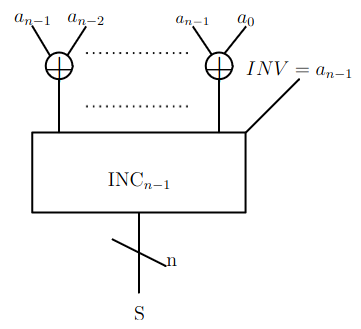
\includegraphics[width=150pt]{figures/Absolute.png}
\end{solutionnoinc}

\begin{solutionnoinc}
    $cost(abs_n)=cost(INC_n-1)+(n-1)\cdot cost(XOR)=(n-1)\cdot cost(HA)+(n-1)$\\ $\qquad\qquad\ \ =3(n-1)$\\\ \\
    Es gibt \textbf{keinen} Überlauf!\quad $|[10...0]|= \langle 10...0\rangle$
\end{solutionnoinc}

\end{frame}

%!Tex Root = ../main.tex
% ./Packete.tex
% ./Design.tex
% ./Deklarationen.tex
% ./Vorbereitung.tex
% ./Aufgabe1.tex
% ./Aufgabe3.tex
% ./Aufgabe4.tex
% ./Appendix.tex

\section{Aufgabe 2}

\setcounter{exercise}{1}


%!Tex Root = ../main.tex
% ./Packete.tex
% ./Design.tex
% ./Deklarationen.tex
% ./Vorbereitung.tex
% ./Aufgabe1.tex
% ./Aufgabe2.tex
% ./Aufgabe4.tex
% ./Appendix.tex

\section{Aufgabe 3}

\setcounter{exercise}{1}

\begin{frame}[allowframebreaks]{Aufgabe \thesection}{Signextension}
  \begin{solutionnoinc}
    \begin{enumerate}
      \item \alert{Zurückführung auf Sign Extension um $1$ Bit:}\\
        \tiny 
        \alert{Lemma:} Sei $a\in\mathbb{B}^n, a = a_{n-1}\ldots a_0$. Dann gilt $[a]_2 = [a_{n-1}a]_2$.\\
        Beweis:\\
        $\displaystyle[a_{n-1}a]_{2}=-a_{n-1}\cdot2^{n}+\sum_{i=0}^{n-i}a_{i}\cdot2^{i}=-a_{n-1}\cdot2^{n}+\left(a_{n-1}\cdot2^{n-1}+\sum_{i=0}^{n-2}a_{i}\cdot2^{i}\right)=-a_{n-1}\cdot2^{n-1}+\sum_{i=0}^{n-2}a_{i}\cdot2^{i}=\left[a\right]_2$\\
        Damit: $[y]_{2}=[y_{n-1}^{1}y]_{2}=[y_{n-1}^{2}y_{n-1}^{1}y]_{2}=\cdot\cdot\cdot=[y_{n-1}^{k}\ldots y_{n-1}^{1}y]_{2}=[\mathrm{sext_{k}}(y)]_{2}.$
    \end{enumerate}
  \end{solutionnoinc}
  \begin{solution}
    \begin{enumerate}
      \item[2.] \alert{Direkter Beweis:}
        \tiny
        Sei $y\in\mathbb{B}^n, y=y_{n-1}\ldots y_0$

        $\begin{aligned}
          {\left[\operatorname{sext}_{\mathrm{k}}(y)\right]_2=[\underbrace{y_{n-1} \ldots y_{n-1}}_{k-m a l}y]_2 } & =\sum_{i=0}^{n-2} y_i \cdot 2^i+\sum_{i=n-1}^{n+k-2} y_{n-1} \cdot 2^i-y_{n-1} \cdot 2^{n+k-1} \\
                                                                                                                   & =\sum_{i=0}^{n-2} y_i \cdot 2^i+y_{n-1} \cdot\left(\sum_{i=0}^{n+k-2} 2^i-\sum_{i=0}^{n-2} 2^i\right)-y_{n-1} \cdot 2^{n+k-1} \\
                                                                                                                   & =\sum_{i=0}^{n-2} y_i \cdot 2^i+y_{n-1} \cdot\left(\frac{2^{n+k-1}-1}{2-1}-\frac{2^{n-1}-1}{2-1}\right)-y_{n-1} \cdot 2^{n+k-1} \\
                                                                                                                   & =\sum_{i=0}^{n-2} y_i \cdot 2^i+y_{n-1} \cdot 2^{n+k-1}-y_{n-1} \cdot 2^{n-1}-y_{n-1} \cdot 2^{n+k-1} \\
                                                                                                                   & =\sum_{i=0}^{n-2} y_i \cdot 2^i-y_{n-1} \cdot 2^{n-1} \\
                                                                                                                   & =[y]_2
        \end{aligned}$
    \end{enumerate}
  \end{solution}
\end{frame}

%!Tex Root = ../main.tex
% ./Packete.tex
% ./Design.tex
% ./Deklarationen.tex
% ./Vorbereitung.tex
% ./Aufgabe1.tex
% ./Aufgabe2.tex
% ./Aufgabe3.tex
% ./Appendix.tex

\section{Aufgabe 4}

\setcounter{exercise}{1}

\begin{frame}[allowframebreaks]{Aufgabe \thesection}{Addition von Zweierkomplementzahlen}
\end{frame}

%!Tex Root = ../main.tex
% ./Packete.tex
% ./Design.tex
% ./Deklarationen.tex
% ./Vorbereitung.tex
% ./Aufgabe1.tex
% ./Aufgabe2.tex
% ./Aufgabe3.tex
% ./Aufgabe4.tex

\section{Appendix}

\begin{frame}[allowframebreaks]{Appendix}{Hinweis zu Hypercubes und Karnaugh Map}
  \begin{itemize}
    \item Wenn sich zwei Knoten nur durch genau $1$ Bit unterscheiden, dann werden sie durch eine Kante verbunden.
  \end{itemize}
  \begin{figure}
      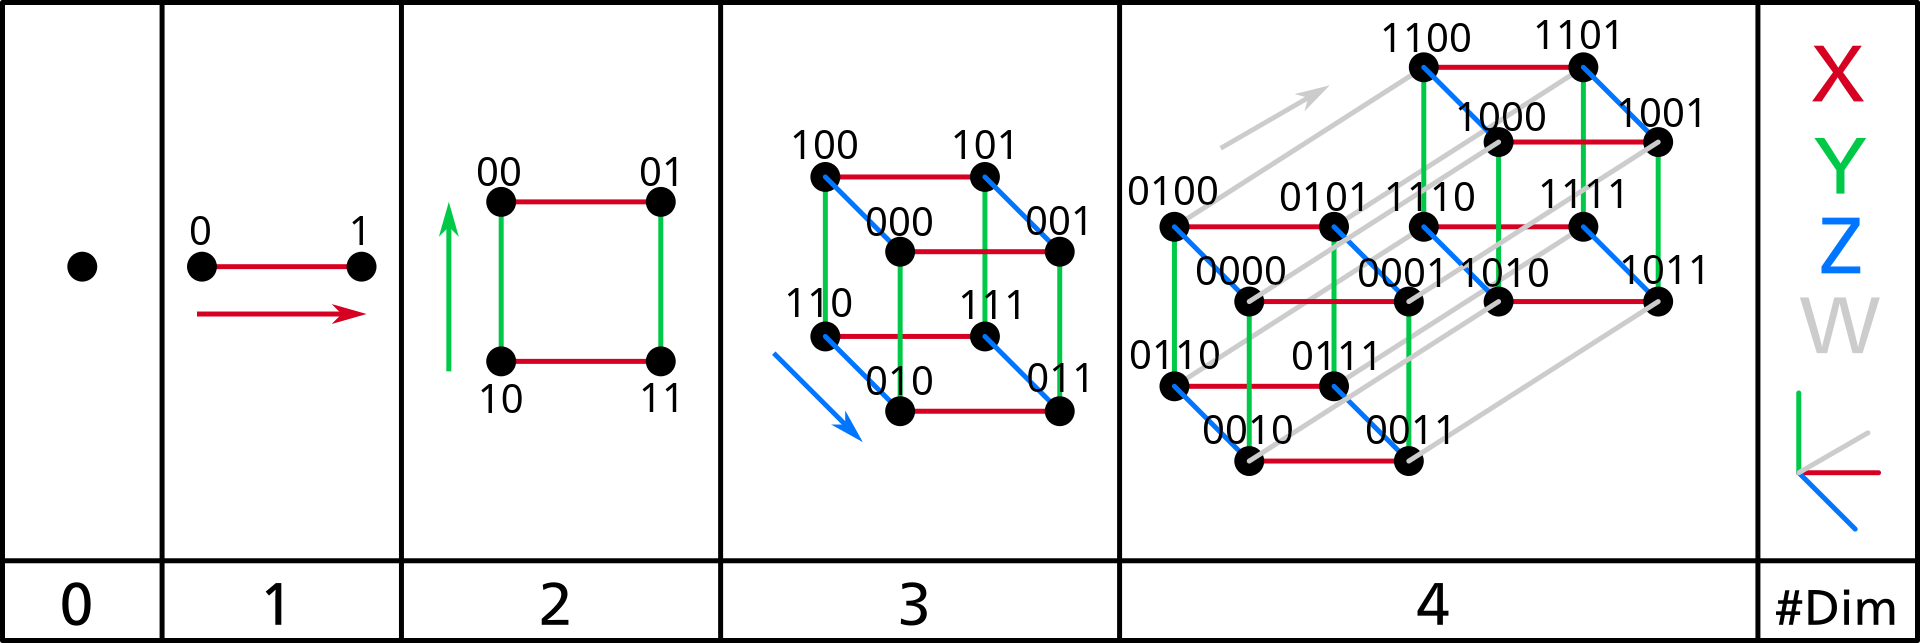
\includegraphics[width=0.8\textwidth, center]{./figures/hypercubes.png}
      \caption{Hypercubes von $n=0$ bis $n=4$}
  \end{figure}
  \newpage
  \begin{figure}
    \centering
    \begin{subfigure}{0.4\textwidth}
       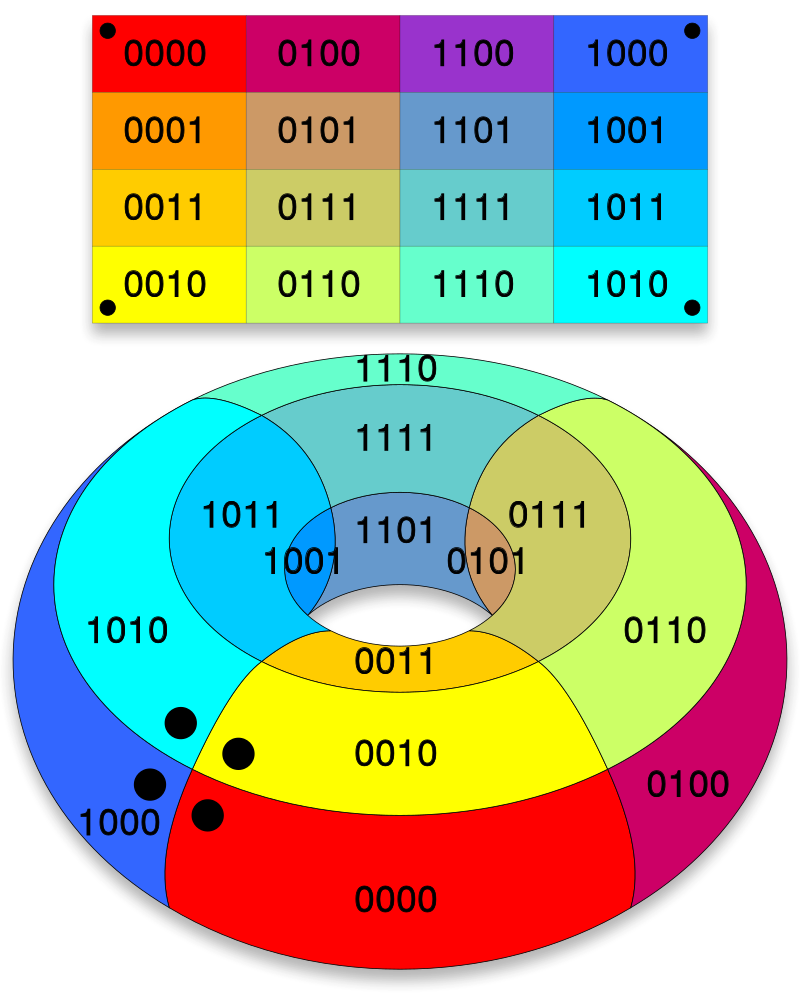
\includegraphics[height=0.4\textheight, center]{./figures/donut.png}
       \caption{Torus oder umgangssprachlich Donut}
    \end{subfigure}
    \begin{subfigure}{0.4\textwidth}
       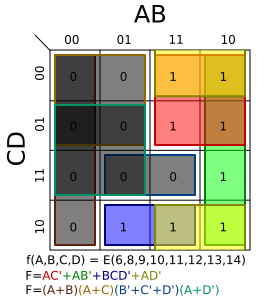
\includegraphics[height=0.4\textheight, center]{./figures/K_map.png}
       \caption{Beispiel für Karnaugh Map}
    \end{subfigure}
  \end{figure}
  \begin{itemize}
      \item Anordnung ist so, weil man einen Hypercube bis $n=4$ (Tesseract) in einer flachen Tabelle darstellen will und im Hypercube gibt es immer nur eine Kante, wenn es nur genau $1$ Bit Unterschied bei $2$ Knoten gibt.
      \item In der Karnaugh Map sind entsprechend immer nur Bitvektoren benachbart, die sich nur in einem Bit unterscheiden. 
      \item Wie bei einem Donut sind Reihen und Spalten miteinander von unten nach oben und von links nach rechts über die Tabelle hinausgehend benachbart.
      \item Von $\overline{a}b$ zu $ab$ gibt es nur $1$ Änderung. Von $\overline{a}b$ zu $a\overline{b}$ gibt es dagegen $2$ Änderungen. Daher sind $\overline{a}b$ und $ab$ benachbart.
  \end{itemize} 
\end{frame}
 

\begin{frame}[allowframebreaks]{Appendix}{Kurzschluss}
  \begin{columns}
    \begin{column}{0.5\textwidth}
      \begin{itemize}
        \item $I=\dfrac{U}{R}$
        \item $P = U\cdot I$
      \end{itemize}
    \end{column}
    \begin{column}{0.5\textwidth}
      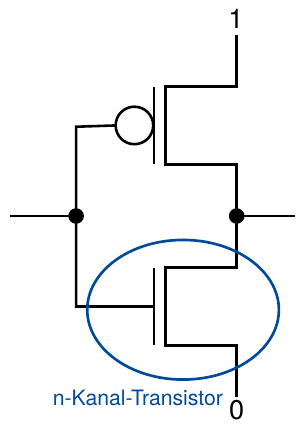
\includegraphics[height=0.6\textheight]{./figures/inverter.png}
    \end{column}
  \end{columns}
\end{frame}

\begin{frame}{Appendix}{Transistoren}
  \begin{itemize}
    \item Ströme steuern. Man kann den Stromfluss innerhalb einer elektrischen Schaltung abbremsen, sodass überhaupt kein Strom fließt (der Transistor funktioniert als Schalter). Man kann aber den Stromfluss auch stark beschleunigen, wodurch ein viel stärkerer Strom fließt (der Transistor funktioniert als Verstärker).
    \item im Kern ist ein Transistor entweder ein strom- oder spannungsgesteuerter Widerstand. Feldeffekttransistoren sind spannungsgesteuerte, Bipolartransistoren sind stromgesteuerte Widerstände.
    \item Unterschiede bei Art der \alert{Lagungsträger}, die zum Stromfluss beiträgt. Bei einem \alert{Bipolartransistor} sind das Elektronen und Löcher. Daher kommt auch der Teil \enquote{Bi} im Namen. Bei einem \alert{Feldeffekttransistor} sind das hingegen entweder Elektronen oder Löcher, also nur eine Art an Ladungsträger.
    \item Feldeffekttransistoren werden überwiegend überall dort verwendet, wo hohe Ströme , Bipolartransistoren hingegen dort, wo geringe Ströme fließen.
  \end{itemize}
\end{frame}

\begin{frame}[allowframebreaks]{Appendix}{Bipolartransistoren}
	\begin{figure}
    \begin{subfigure}{0.4\textwidth}
      \centering
      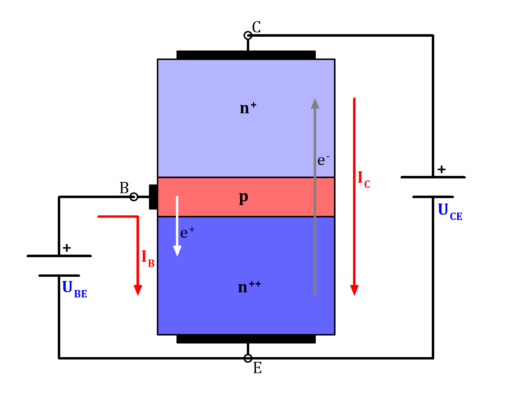
\includegraphics[height=0.5\textheight]{figures/pnp-Transistor}
      \caption{PNP-Transistor}
      \label{fig:pnp-transistor}
    \end{subfigure}
    \begin{subfigure}{0.4\textwidth}
      \centering
      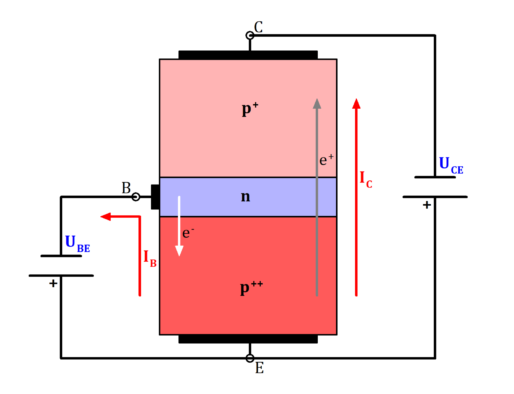
\includegraphics[height=0.5\textheight]{figures/npn-Transistor}
      \caption{npn-Transistor}
      \label{fig:npn-transistor}
    \end{subfigure}
	\end{figure}
  \begin{itemize}
    \item \alert{drei Anschlüsse:} Collector (C), Base (B) und Emitter (E)
  \end{itemize}
\end{frame}

\begin{frame}[allowframebreaks]{Appendix}{Feldeffekttransistoren}
  \begin{figure}
    % \begin{subfigure}{0.4\textwidth}
      \centering
      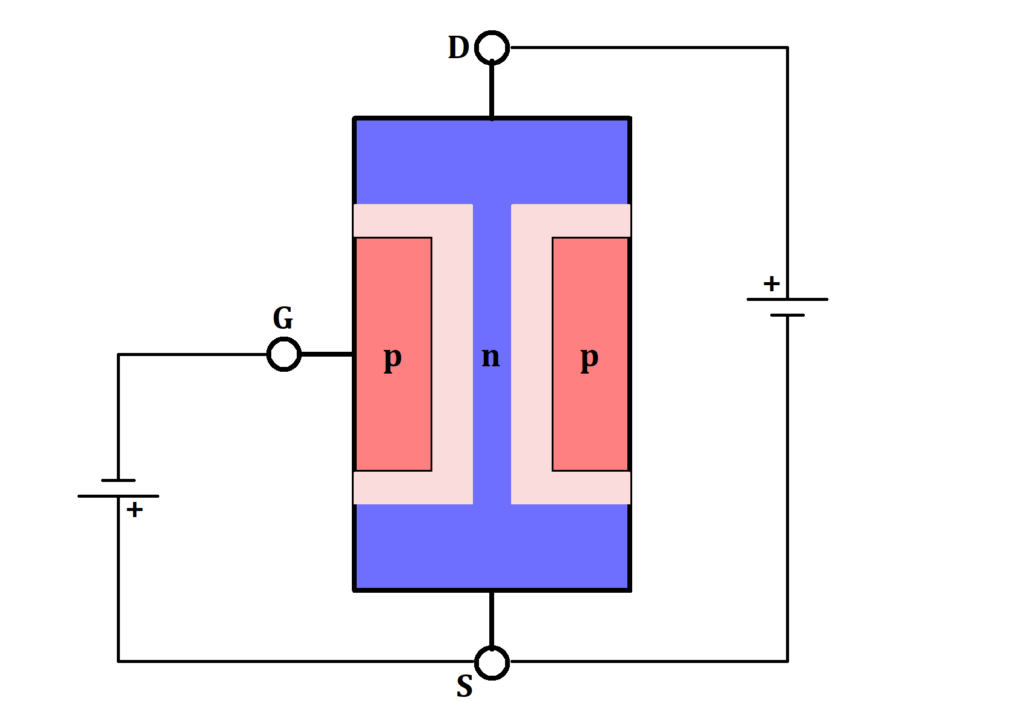
\includegraphics[height=0.5\textheight]{figures/n-Kanal-Feldeffekttransistor.png}
      \caption{n-Kanal-Feldeffekttransistor}
    % \end{subfigure}
    % \begin{subfigure}{0.4\textwidth}
    %   \centering
    %   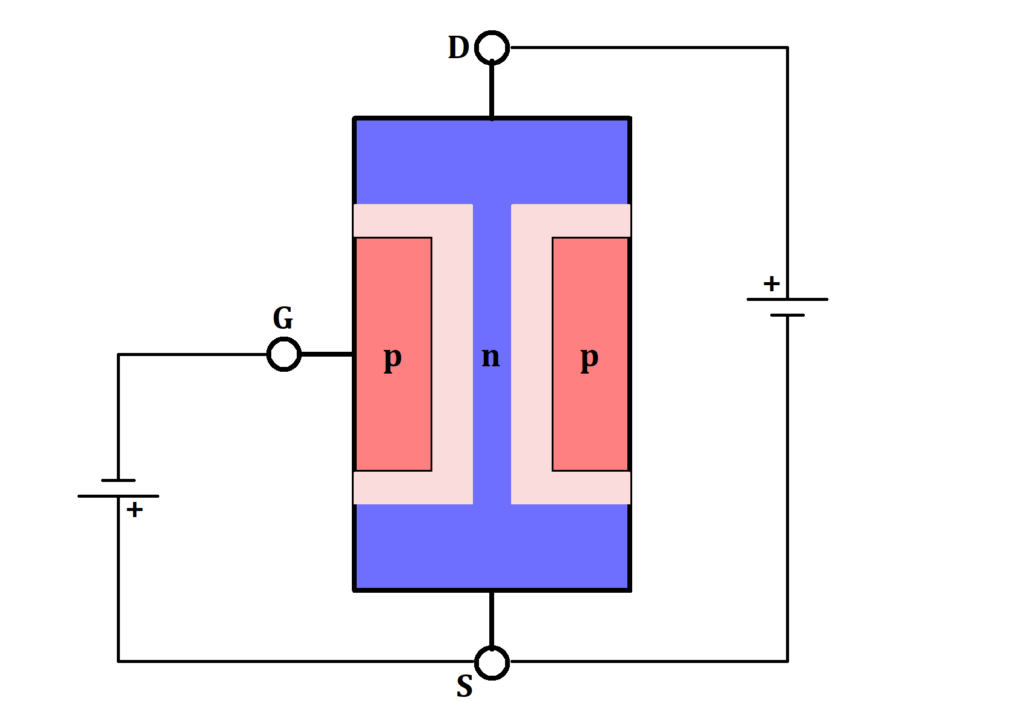
\includegraphics[height=0.5\textheight]{figures/n-Kanal-Feldeffekttransistor.png}
    %   \caption{p-Kanal-Feldeffekttransistor}
    % \end{subfigure}
  \end{figure}
  \begin{itemize}
    \item \alert{drei Anschlüsse:} Drain (D, \enquote{Senke, Abfluss}), Gate (G, \enquote{Tor}) und Source (S, \enquote{Quelle, Zufluss})
    \item Sperrschicht-Feldeffekttransistor (SFET, engl. JFET)
    \item Je nachdem wie der Kanal, durch denen die Ladungsträger fließen, dotiert ist, findest man die Bezeichnungen n-Kanal-FFET und p-Kanal-FFET
  \end{itemize}
\end{frame}

% % Beweis Euklidischer Algorithmus
% diese allgemeine mit Wertigkeit usw.
% Wie N- und P-Kanal-Transistoren funktionieren
% Polynomring
% Übersicht Implikation
% Methematische Logik, a und ~a, a oder ~a
% Necessary and Sufficient, Beiespiel mit Kurvenkdiskussion
% Modelle, Strukturen, Quantoren Bild
% RETI ist eine Register-Memory Architektur, Accumulator Architektur
% es gibt Kontrollsignale und die anderen Signale
% wie Hypercubes genau funktionieren

% Emails werden noch beantwortet
% in welcher Reihenfolge am sinnvollsten bearbeiten?
% Klarstellung Begriff Boolesche Algebra
% surjektiv bezüglich Bildmenge ist sowieso klar, deswegen spricht man es nicht aus, aber ja stimmt
% wie sich das Binärsystem für Kommastellen fortsetzt mit 2^{-1}
% bei KNF und Karnaugh Map muss man immer von der negierten Maxtermen ausgehen bei eintragen in die Tabelle. Wobei es einfach ausgedrückt einfach die Invertierung der anderen Tabelle ist
% wie man sich P-Kanal und N-Kanal gut merken kann, p und 0, N und I und lässt genau dann durch, wenn es 0 ist
% die Sache mit 11111 möglichst große Zahl

%!Tex Root = ../main.tex
% ./Packete.tex
% ./Design.tex
% ./Deklarationen.tex
% ./Vorbereitung.tex
% ./Aufgabe1.tex
% ./Aufgabe2.tex
% ./Aufgabe3.tex
% ./Aufgabe4.tex

\section{Bonus}

\begin{frame}[allowframebreaks]{Bonus}{Vollständige Induktion über natürliche Zahlen\vspace{0.5cm}}
  \begin{itemize}
    \item für \alert{Allbehauptungen}: $\forall n\in\mathbb{N}:\mathcal{E}(n)$ (Eigenschaft $\mathcal{E}$)
    \item die allgemeine Form wird als \alert{Strukturelle Induktion} bezeichnet, \alert{Vollständige Induktion} ist zum Beweis von Aussagen für alle Natürlichen Zahlen
    \begin{itemize}
      \item Menge der \alert{natürlichen Zahlen} $\mathbb{N}$ weißt geignete Struktur auf, da auf ihnen die Nachfolgerbeziehung besteht
    \end{itemize}
    \item man führt Teilbewise für $2$ Fälle: 
    \begin{itemize}
      \item \alert{Basisfall:} ${\mathcal{E}}(0)$, d.h. die natürliche Zahl $0$ hat die Eigenschaft $\epsilon$
      \item \alert{Induktionsfall:} $\forall i\in\mathbb{N} \left(\mathcal{E}(i)\Rightarrow\mathcal{E}(i+1)\right)$, d.h. die Eigenschaft $\epsilon$ überträgt sich von jeder natürlichen Zahl $i$ auf ihren Nachfolger $i + 1$
    \end{itemize}
    \item bei beweisender Allbehauptung für den Induktionsfall wird Implikation: Sei $i\in\mathbb{N}$ beliebig. Zu zeigen: $\epsilon(i)\Rightarrow\epsilon(i+1)$ zerlegt in: Sei $i\in\mathbb{N}$ beliebig. Es gelte: $\epsilon(i)$. Zu zeigen: $\epsilon(i+1)$
    \item Diese Darstellung des Induktionsfalls legt seine Zerlegung in die üblichen drei Bestandteile \alert{Induktionsannahme}, \alert{Induktionsbehauptung}, \alert{Induktionsschritt} nahe:
  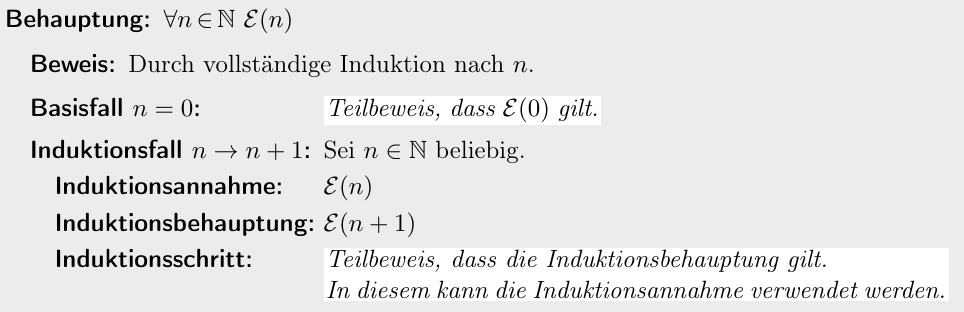
\includegraphics[width=\linewidth]{./figures/vollstaendige_induktion.png}
  \end{itemize}
  \begin{itemize}
    \item Induktionsfall beweist Allbehauptung mit darin enthaltener Implikationsbehauptung 
    \item Wenn für Eigenschaft $\epsilon$ Basisfall und Induktionsfall bewiesen sind, gilt, dass jede natürliche Zahl die Eigenschaft $\epsilon$ hat, denn:
    \begin{enumerate}
      \setcounter{enumi}{-1}
      \item Wegen des Basisfalls gilt $\epsilon(0)$.
      \item Mit $\epsilon(0)$ gilt wegen des Induktionsfalls auch $\epsilon(1)$.
      \item Mit $\epsilon(1)$ gilt wegen des Induktionsfalls auch $\epsilon(2)$.
      \item Mit $\epsilon(2)$ gilt wegen des Induktionsfalls auch $\epsilon(3)$.
      \item $\ldots$
    \end{enumerate}
  \end{itemize}
  \includegraphics[width=0.6\textwidth]{./figures/vollständige_induktion_1.png}
  \includegraphics[width=0.8\textwidth]{./figures/vollständige_induktion_2.png}
\end{frame}

\begin{frame}[allowframebreaks]{Bonus}{O-Notation}
  \begin{itemize}
    \item Man will Funktionen irendwie vergleichen und das einzige sinnvolle was man vergleichen kann ist die \alert{Wachstumsrate}, denn für zwei Funktionen kann gleichzeitig gelten: $g = O(f)$, also $g$ wächst nicht stärker als $f$ und $g > f$, also $g$ ist überall echt größer als $f$
    \item Konstate Faktoren und Summanden $c \cdot x$ und $c + x$ sollen keine Rolle, aber es geht um \alert{Wachstumsrate}, Konstante Faktoren und Summanden spielen keine Rolle
    \item Die Operatoren $O, \Omega, \Theta, o, \omega$ sind auf Funktionen, was die Operatoren $\le, \ge, =, <, >$ auf Zahlen sind
    \item man sagt die \enquote{Laufzeit eines Algorihmus ist: $\Omega(n\cdot log(n))$}, man sagt \alert{NICHT}, dass ein \enquote{Algorithmus Laufzeit mindestens $O(n\cdot log(n))$ hat}
    \item \alert{formal:} 
    \begin{itemize}
      \item $O(f)= \{g: \mathbb{N}\to\mathbb{R} | \exists n_0\in\mathbb{N}, \exists C > 0, \forall n\ge n_0, g(n)\le C \cdot f(n)\}$
      \item $\Omega(f)= \{g: \mathbb{N}\to\mathbb{R} | \exists n_0\in\mathbb{N}, \exists C > 0, \forall n\ge n_0, g(n)\ge C \cdot f(n)\}$
    \end{itemize}
    \item \alert{Bestimmung über Grenzwerte:}
    \begin{enumerate}
      \item $\displaystyle f=O(g) \Leftrightarrow \operatorname{lim}_{n\to\infty}\frac{f(n)}{g(n)} < \infty$
      \item $\displaystyle f=\Omega(g) \Leftrightarrow \operatorname{lim}_{n\to\infty}\frac{f(n)}{g(n)} > 0$
      \item $\displaystyle f=\Theta(g) \Leftrightarrow \operatorname{lim}_{n\to\infty}\frac{f(n)}{g(n)} > 0$ und $\displaystyle\operatorname{lim}_{n\to\infty}\frac{f(n)}{g(n)} < \infty$
      \item $\displaystyle f=o(g) \Leftrightarrow \operatorname{lim}_{n\to\infty}\frac{f(n)}{g(n)} = 0$
      \item $\displaystyle f=\omega(g) \Leftrightarrow \operatorname{lim}_{n\to\infty}\frac{f(n)}{g(n)} = \infty$
    \end{enumerate}
  \end{itemize}
\end{frame}

\begin{frame}{Bonus}{Regel von L'Hopital}
  \begin{itemize}
    \item $\displaystyle \operatorname*{lim}_{x\to c}{\frac{f(x)}{g(x)}}=\operatorname*{lim}_{x\to c}{\frac{f^{\prime}(x)}{g^{\prime}(x)}}$
    \begin{itemize}
      \item wird verwendet bei Grenzwertbetrachtung bei der man bei Zähler und Nenner entweder den Fall $\frac{0}{0}$ oder $\frac{\pm\infty}{\pm\infty}$ hat und beide Ableitungen differenzierbar % und $g(x)\ne 0$ für $x\ne y$ für den Fall $\frac{0}{0}$ und $g(x)'\ne 0$ für den Fall $\frac{\infty}{\infty}$ 
      \item dann Zähler und Nenner des Bruches getrennt voneinander ableiten und dann nochmal Grenwertbetrachtung
      \item wenn nochmal unbestimmter Ausdruck rauskommt und wieder entweder der Fall $\frac{0}{0}$ oder $\frac{\infty}{\infty}$ und beide Ableitungen differenzierbar, dann nochmal anwenden oder sonst Pech gehabt
    \end{itemize}
  \end{itemize}
\end{frame}


% \section{Literatur}
%
% \begin{frame}{Bücher}
%   \printbibliography[type=book,heading=subbibliography,title={Bücher}]
% \end{frame}
%
% \begin{frame}{Artikel}
%   \printbibliography[type=article,heading=subbibliography,title={Artikel}]
% \end{frame}
%
% \begin{frame}{Vorlesungen}
%   \printbibliography[type=unpublished,heading=subbibliography,title={Vorlesungen}]
% \end{frame}
%
% \begin{frame}{Online}
%   \nocite{noauthor_filehandshake_2020}
%   \printbibliography[type=online,heading=subbibliography,title={Online}]
% \end{frame}
%
% \begin{frame}{Sonstiges}
%   % \printbibliography[nottype=book, nottype=article, nottype=online, nottype=unpublished,heading=subbibliography,keyword=wikikeyword,title={Sonstige Quellen}]
%   \printbibliography[nottype=book, nottype=article, nottype=online, nottype=unpublished,heading=subbibliography,title={Sonstige Quellen}]
% \end{frame}
\end{document}
